s\documentclass[10pt]{article}
\usepackage[pdftex]{graphicx}
\usepackage{indentfirst}

\pdfpagewidth 8.5in
\pdfpageheight 11in

\setlength\topmargin{0in}
\setlength\headheight{0in}
\setlength\headsep{0in}
\setlength\textheight{8in}
\setlength\textwidth{6.5in}
\setlength\oddsidemargin{0.2in}
\setlength\evensidemargin{0.2in}
\setlength\parindent{0.25in}
\setlength\parskip{0.035in} 

\title{BarraCUDA Project: A Homebrew Supercomputer}
\author{Matt Redmond}
\date{3 April 2010}
\begin{document}

\maketitle
\section{Abstract}
The BarraCUDA (Beginner's Analytic Research and Rendering Architecture over C Unified Device Architecture) project will ultimately entail a small-scale homebrew supercomputer designed around the NVIDIA CUDA architecture, as well as a physical simulation of electrodynamics coded to take advantage of this CUDA architecture. The project is meant to serve as an introductory platform for student-researchers to develop parallel-programming skills, and design programs that showcase concepts in modern science research through real-time visualization. This project will explore the vast world of scientific computing through the lens of a physicist, and should provide ample opportunities to learn new techniques in computational physics as well as numerical analysis.
\begin{figure}[h]
	\centering
		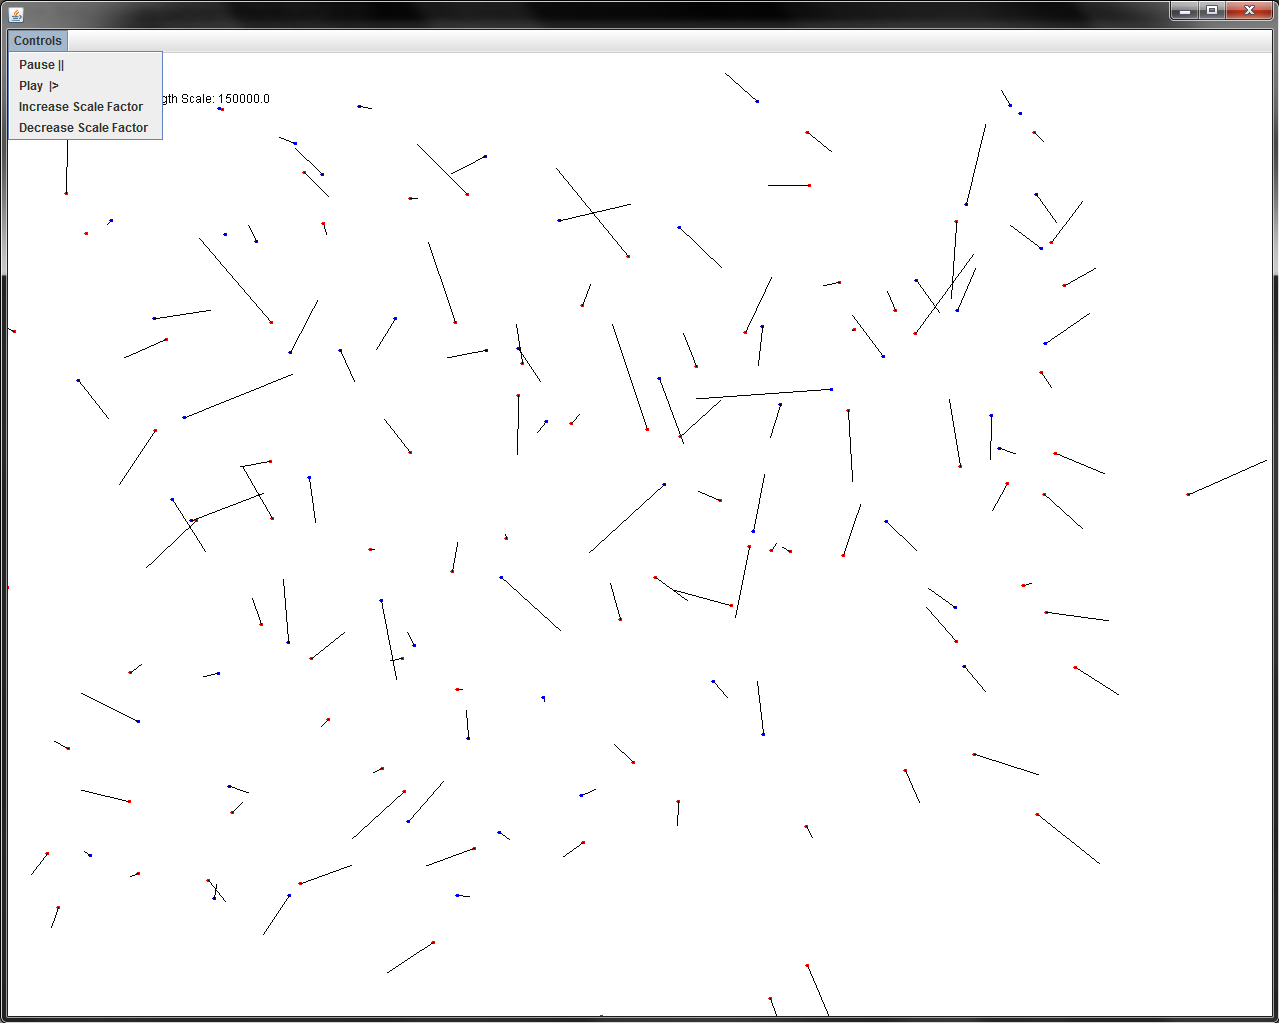
\includegraphics[scale = 0.35]{barracuda2DScreenshot.png}
	\caption{A screenshot of the simulation in action.}
	\label{fig:barracuda2DScreenshot}
\end{figure}

\clearpage
\tableofcontents
\clearpage
\section{Introduction} %why is this interesting to explore?
Through his Applied Science Research and Computer Science classes, the author has gradually become aware of the growing importance of high performance computational power in the fields of physical, chemical, and biological research. A small sample of these problems can be found at http:// www.nvidia.com/object /cudahome.html, but three particularly interesting ones (that form a representative sample of the types of problems that one can approach with supercomputing resources) are [1], [2], and [3]. Ultimately, the author is interested in learning more about visual representations of physical modeling problems, but recently, the author got a chance to work in Caltech's materials physics lab on the DANSE project, using distributed computational analysis to model the theoretical results of neutron scattering experiments before actually conducting them. It was here where the author was exposed to the elegant concept and power of a Beowulf cluster. He realized that high schools could make good use of such a powerful tool (on a smaller scale) for instructional purposes, in the demonstration/visualization of scientific concepts as well as the programming process.

The author designed a simulation of electrodynamics on a CUDA-based supercomputer because CUDA represents the new direction that high performance computing is moving in: instead of waiting for a single fast central processing unit to perform heavy calculations sequentially, these calculations are farmed out in parallel to hundreds of individual graphics processing unit cores for computation. The actual performance increase (across diverse applications) is reported by various sources [4] to be anything from 5x to 2600x faster than a CPU-based system. Furthermore, the CUDA architecture is alive and well-supported by the community, with various development tools available, and many new applications released frequently. CUDA supports the API OpenMP, a well-known parallel processing API that is widely supported in the scientific computing community. CUDA is supported on several chipsets, but the two most suitable consumer-grade architectures for this project are the NVIDIA GeForce GTX295 and the NVIDIA Tesla C1060. 

The bottom line: supercomputing as a field continues to grow very rapidly, and most pure sciences are relying upon it to provide a foundational basis for carrying out their research. It's particularly interesting to explore the underpinnings of graphics processor based supercomputing, because the onset of GPU computing provides a brand new avenue for massive scalability that simply isn't present under the CPU-based paradigm.


\section{History}
Supercomputing has come a long way from its origins. The growth of supercomputing has historically mirrored the growth of CPUs, following the famous Moore's Law, which stipulates that available processing power doubles roughly every 18 months. The very earliest supercomputers (notably, the Cray-1) were designed as vector processors, intended to process instructions in parallel by employing tricks like unrolling loops and managing memory in tuples. [5] These vector processors provided the very first approach to true parallelism, but were distinct from modern parallel processors in that they only had one core CPU. The Cray-1 had an effective computation speed of 160 MFlops, which was worth \$8,000,000 to various government corporations in the '70s. Today, the most powerful supercomputers are tracked by a 3rd party website (www.top500.org). The top computer on this list is the Cray XT5HE Jaguar at Oak Ridge National Laboratory, with 224,162 cores and a benchmarked performance of 1,759 TFlops, nearly 11 million times faster than the Cray-1 [6]. As computing resources have improved over time, the complexity of the problems that we are able to investigate has scaled up. While the initial Cray-1 was used for making 10-day weather forecasts faster [7], the newest supercomputers are used for things like modelling the interaction between individual molecules of a complex protein, or investigating the geological properties of tectonic plates. 


\section{Theory}

\subsection{Supercomputing Theory}
A GPU-based supercomputer differs from standard CPU-based supercomputers in a number of ways: the most obvious one of these is the actual location and type of the numerical processors. A CPU-based cluster (Supercomputers and cluster computers will be mentioned interchangeably in this paper; they are equivalent for our purposes) uses processors housed directly on the node motherboard, which communicate directly with the system memory through a high-speed bus. This has the advantage of extremely fast memory read/write operations, but it has the disadvantage (currently) of a relatively small number of available cores for processing. CPU based implementations also have issues recycling computations for fewer wasted cycles. The current top-of-the-line Intel i7-920 runs 8 cores at 1600 MHz each [8]. The GPU, in comparison, resides (generally) in an interface bus. In modern computers, this bus is the PCI express bus, which provides an indirect way of communicating with the memory through a controller chip on the motherboard. The advantage of the GPU-based system is that it can run many more cores than a CPU-based system can (240 cores per card in the BarraCUDA system at 1242 MHz each) [9], but the disadvantage is that it has relatively slower memory read/write times. Most GPUs attempt to deal with this by including memory onboard the card (4 GB in the BarraCUDA system per card), so the read/write times are reduced to those of a CPU-based system. As one can see, there are significant advantages to using a GPU-based setup.

The main advantage (having drastically more cores) of the GPU-based system is made most clear when a program is designed to UTILIZE all of those cores in parallel. Certain problems lend themselves well to this paradigm; others do not. An example of an easily parallelizable problem is one that can be broken down into a number of sub-tasks, each of which can be computed independently of the other tasks. The n-body electrodynamics problem is a perfect example of an easily parallelizable problem: computing the force on each particle at a given timestep only relies on the previous position of all of the other particles. If we store the point charge positions in an array that is globally accessible by all of the cores, then we can update each particle SIMULTANEOUSLY. This is a HUGE speedup over the sequential calculations enacted by a single-core CPU setup, and provides the motivation for a multiple-core setup in general.

\clearpage
\subsection{Scientific Theory}
The simulation that is currently in place relies upon Coulomb's Law to generate the electric field acting on each individual point charge. This efield generates a force that is similar to the gravitional force in that it is an inverse-square law, but different because the force vector is signed (instead of always attracting like gravity, it can attract or repel). The force vector acting on a point charge is represented by $\vec{F} = q\vec{E}$, where $q$ is the charge of the particle and $\vec{E}$ is the electric field acting on the particle. The explicit way to compute $\vec{E}$ is to sum up the effects of each other particle in the simulation on the particle in question.

Coulomb's Law gives this electric field sum as $$\vec{E} = \frac{1}{4\pi\epsilon_0}\sum_{i = 1}^n \frac{q_i (\vec{r} - \vec{r_i})}{|\vec{r} - \vec{r_i}|^3}$$ where $\vec{r}$ is the vector to the point that we are testing the electric field at, and $\vec{r_i}$ is the vector of the point we are testing against. As $i$ ranges from $1$ to $n$, we test the electric field against all other particles. This means that updating ONE particle's electric field requires us to check $n-1$ other particle's states, where $n$ is the total number of particles. Updating ALL of the particle's electric fields requires $n(n-1)$ checks, making the n-body electrodynamic simulation a problem known as an $O(n^2)$ problem (it has time complexity asymptotically equal to some constant multiple of $n^2$). These problems scale notoriously badly on standard PC hardware, but with a supercomputer, they become approachable again. There are ways to speed this problem up (by only considering particles within a certain distance of each other to have an observable effect) which can reduce the runtime complexity, but these methods trade a gain in speed for a reduction in accuracy.

Coulomb's Law is derived under the assumption that the particles are stationary. When they are moving, Coulomb's Law provides only an approximation to the electric field acting on the particles. In motion, these particle actually generate electromagnetic waves that can perturb the electric field of the others. For this simulation, however, Coulomb's Law is the only formula used to compute the forces on the particles. Furthermore, the scale factor $\frac{1}{4\pi\epsilon_0}$ is roughly equal to $9 \times 10^9$, which is too large for accurate computation. Because $\epsilon_0$ is defined as $\frac{1}{\mu_0 c^2}$, where $c$ is the speed of light and $\mu_0$ is the magnetic constant (generally defined as $4\pi \times 10^{-7} \frac{H}{m}$), these values are all system-unit dependent. To counter this, a system of units that is normalized to the electron mass, charge, and radius was implemented, so this constant scale factor $\frac{1}{4\pi\epsilon_0}$ is absorbed into the graphics engine.

The integrator written for this project is (essentially) a numeric differential equation solver. This integrator uses the Runge-Kutta 4 method, which works by exploiting Euler's method: RK4 reduces the magnitude of the error term by sampling the derivatives four times over the timestep interval. A general introduction to this technique is given at [10], and indeed, the author's technique has been adapted for this particular implementation. This integrator has average error on the order of $O(n^5)$, which provides a tradeoff between speed and accuracy. It can also correctly model situations where two particles are very close together, as the reduced error term (and weighted sum of derivatives) is much more robust under the influence of large outliers than Euler's method is.

\clearpage
\section{Algorithm Implementations}
Initially, the simulation was conducted as a pure $O(n^2)$ algorithm using the exact, derived form of Coulomb's law to determine the force acting on each particle. This is the most rudimentary simulation possible, and although it is fairly straightforward to implement, it leaves many things to be desired. First, this implementation is remarkably slow when run on systems of particles $N > 250$, which is an unacceptably low threshold. Second, this implementation has great difficulty processing particles that are situated very close together. To test the numerical stability of the first implementation's solutions, a conservation-of-momentum test was run, with results available in the second appendix. Because the collision response code is fully elastic, linear momentum should be conserved between any two timesteps. Ideally, the total momentum vector of the system will remain at $<0, 0, 0>$, but this is not the case in practice. The first implementation ($O(n^2)$ w/o perturbation) produced a series of momenta vectors that fluctuated wildly between timesteps when a lot of collisions were ocurring. This fluctuation was quantified by a metric of $|1 - \frac{T(i+1)}{T(i)}|$, where T(i) represents the total momentum at timestep $i$. This metric treats negative momentum change equivalently to positive momentum change, and allows us to average the momentum changes over an entire trial run. To combat the accumulation of integration errors on close-proximity particles, a ``perturbation'' was added into the denominator of Coulomb's Law, as per [11]. Coulomb's Law transforms into

$$\vec{E} = \frac{1}{4\pi\epsilon_0}\sum_{i = 1}^n \frac{q_i (\vec{r} - \vec{r_i})}{(|\vec{r} - \vec{r_i}| + \epsilon)^3}$$ 

\begin{figure}[ht]
	\centering
		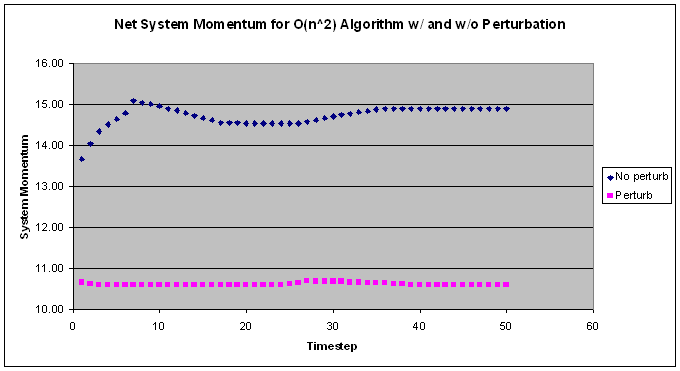
\includegraphics[scale = 0.75]{graphOfPerturbMomentum.PNG}
	\caption{This graph displays the total momentum of a system of particles (N = 150) over 50 timesteps.}
	\label{fig:graphOfPerturbMomentum}
\end{figure}

This perturbation by $\epsilon$ reduces the effect of division by an arbitrarily small distance, but also reduces the accuracy of the simulation. The larger the perturbation is, the more "safe" the system is from integration error. Unfortunately, physical accuracy also decreases as the perturbation increases. In this simulation, $\epsilon = 10^{-12}$. This perturbation, when applied to the $O(n^2)$ algorithm, produces a markedly large effect on numerical stability, as visible from the data in the second appendix. The perturbation method implemented here comes out as the clear stability champion, reducing the momentum fluctuations by nearly 85\% in the average case between timesteps. The average numerical error can similarly be computed for each implementation by dividing the average delta momentum per timestep by the average total momentum per timestep. For the implementation without perturbation, the average error is $0.000225274$, and for the implementation with perturbation, the average error is $4.9066 \times 10^{-5}$

\section{Algorithm Speed}
Although this perturbation handles the numerical stability of the solution, it does nothing to address the speed of the algorithm. A clever algorithm by Barnes and Hut [12] makes use of a special octtree data structure to reduce the problem to $O(n \log n)$, at the expense of physical accuracy. This structure separates space recursively, through the use of splitting planes. It divides all of space into octants, then divides each of these octants into octants, and so on. This recursive data structure is stored as a tree, with a root having 8 leaves, and each leaf has 8 children. This manner of storage is continued until each point resides in its own node of space. The data structure has as many nodes as there are point charges. The clever idea presented by Barnes and Hut is to use the $O(n^2)$ algorithm for every leaf-node ``close to'' the node under consideration, but treat all other nodes as a single, far away charge (composed of a superposition of these other nodes). This is tenable because the inverse square law is less sensitive to error when the points under consideration are far away. The Barnes-Hut algorithm trades off a MUCH faster speed for reduced accuracy. This algorithm essentially treats far away charges as a ``single pole,'' and is generally within 1\% accuracy of the exact $O(n^2)$ pair-wise algorithm. If this algorithm's precision is too low, there exists a seperate $O(n \log n)$ algorithm known as the ``Fast Multipole Model'' (FMM). This method is similar to Barnes-Hut, but does not condense ALL other far particles into a single pole particle. Instead, it makes tradeoffs and condenses some of the nodes into single poles, but leaves these poles collected at the centroid of their respective layers. It condenses the far away points into a few separated single poles. This method is still $O(n \log n)$, but has a worse scaling factor in practice.

These algorithms are clearly suited to parallelization because their data structures promote shared memory usage and recycled calculations. The centroid for the multipoles can be held in memory (it doesn't need to be recomputed each time a layer is evaluated), and each particle can run a multi-pole condensation on its own thread. 

After implementing a Fast Multipole algorithm, the author noticed a few things: on systems of particles smaller than about 1500 particles, the $O(n^2)$ algorithm is substantially faster than the $O(n \log n)$ algorithm by a considerable margin. This is likely due to the overhead required for the FMM algorithm to work: tree construction, recursive information summary, and integration are a lot more complicated on a spatially-indexed data structure. The tree operations are a lot more expensive, although the force-computing method is cheaper. The author intends to tune the FMM model in the coming month to meet or exceed the performance of the naive $O(n^2)$ algorithm. Until then, the performance hit is too large to provide a valid comparison between the two algorithms. Data will be forthcoming in the future month, as well as a table comparing the precision and speed of the two implementations.

\clearpage
\section{Accomplishments}
Currently, the simulation is able to display two-dimensional interactions between charged particles. The underlying engine is actually processing the vectors as three-dimensional vectors, but three-dimensional graphics haven't been implemented yet. A fully functional Runge-Kutta4 numerical integrator is coded in the NumericalIntegration.java file. The graphics are rudimentary at the moment, but they provide a decent visual for what is happening with the particles. The user can toggle the momentum and efield vectors on and off inside of the twoDimensionalSim.java file by commenting and uncommenting the code. The simulation can be paused, and particles (of various charges) can be added upon mouseclick. A lot of the actual explanation for what is being done is provided inside of the code as comments. The simulation is currently running an $O(n \log n)$ algorithm with perturbation, though this implementation seems to be considerably slower than the previous $O(n^2)$ algorithm. A lot of the source code has been cleaned up since the original implementation: many of the initialization methods have been combined into one method, and a lot of the data structures that were being passed back and forth were eliminated. This leads to a smaller memory footprint, and ultimately a faster program.

\section{The Next Steps}
\subsection{For February}
Fixing collision detection is a short term goal, but a longer term goal is getting three dimensional graphics set up. I'll probably use the OpenGL standard graphics library, or whatever the CUDA IDE provides, as a test bed. Finally, I still need to find a way to interface the simulation (I am looking at a library called JCUDA for this) and parallelize the numerical calculation so that is it suitable for use with the CUDA architecture. As described in the Scientific Theory section, the algorithm is easily parallelized, but the actual low-level core operation might not be. I'll spend some time looking through CUDA documentation and working with OpenMP. 

I have a CUDA-enabled testbed that I will experiment on, and the next highest priority in this project will become the migration of the simulation code to CUDA code. It's likely that this will be fraught with errors, and will require substantial amounts of debugging, but I hope to have the simulation migrated in about a month. The parallelization will require ongoing effort to optimize, but the initial setup should be fairly straightforward. There are a lot of places that this project can go, from increased accuracy to higher speed, to modelling more complicated approximations, and I look forward to approaching all of these avenues.

\subsection{For March}
I'm also going to migrate to the FMM algorithm soon, and should see a noticeable increase in computation speed. I'll have to work out a metric that lets me determine that physical modeling inaccuracy, but this would require that I *know* the exact solution. I'll look through the literature to check how other researchers evaluate the physical accuracy of their methods. This FMM algorithm can be adapted to arbitrary precision, so if the precision becomes noticeably bad, it is easily correctable. I'm still looking to migrate onto CUDA soon, but it appears that I will need to read more in depth about how CUDA handles shared memory. The memory access part of asynchronous threads seems to be the most difficult part to implement properly. Collision detection has been handled (more or less) by implementing the perturbation to Coulomb's Law. I've been doing a lot of reading on OpenGL interaction with CUDA, and that will be the third step. The new chronology is now 1) Get Parallel-FMM implemented. 2) Migrate to CUDA + Shared Memory. 3) Implement JOGL Graphics/Visualization Software.

\subsection{For April}
Parallel-FMM is taking longer than expected to implement correctly. It is likely that this will take considerably more effort to finish. CUDA support will be implemented at a later date. It is unlikely that fully three dimensional graphics will be implemented under the current time frame. Parallization shouldn't be quite as complicated (once the FMM model is in place) because I can simply assign each core a different root node of a tree to handle. This could be done in as few as ten lines of code, from preliminary investigations. 

\section{Citations}


\begin{verbatim}
[1] CUDA-Based Incompressible Navier-Stokes Solver. Julien Thibault and Inanc Senocak.
<http://coen.boisestate.edu/senocak/files/BSU_CUDA_Res_v5.pdf>

[2] TeraFlop Computing on a Desktop PC with GPUs for 3D CDF. J. Tolke and  M. Krafczyk.  
<http://www.irmb.bau.tu-bs.de/UPLOADS/toelke/Publication/toelkeD3Q13.pdf>

[3] CUDA Acceleration of Molecular Dynamics. David Kirk and Wen-mei W. Hwu.  
<http://www.ks.uiuc.edu/Research/gpu/files/lecture8casestudies.pdf>

[4] NVIDIA CUDA Project Repository. <http://www.nvidia.com/object/cuda_home.html#>

[5] Matlis, Jan. A Brief History of Supercomputers. 
<http://www.cio.com.au/article/132504/brief_history_supercomputers>

[6] Cray XT5HE Jaguar Specifications. <http://www.top500.org/system/10184>

[7] Cray Corporation History. <http://www.cray.com/About/History.aspx>

[8] Intel Core i7 Specifications <http://www.intel.com/products/processor/corei7/specifications.htm>

[9] NVIDIA GTX295 Specifications <http://www.nvidia.com/object/product_geforce_gtx_295_us.html>

[10] Fiedler, Glenn. Physics in 3D. <http://gafferongames.com/game-physics/physics-in-3d/>

[11] Nyland, Lars. Harris, Mark. Prins, Jan. Fast N-Body Simulation with CUDA. 
<http://wwwx.cs.unc.edu/~prins/Classes/633/Readings/nbody_gems3_ch31.pdf>

[12] CS267 Lecture Notes: 11 April 1996. Fast Hierarchical Methods for the N-body Problem.
<http://www.cs.berkeley.edu/~demmel/cs267/lecture26/lecture26.html>
\end{verbatim}

\clearpage
\section{Additional Sources}
\begin{verbatim}
Chen, Y. Chen, Nicholas. Barnes-Hut N Body Simulation. 
<https://agora.cs.illinois.edu/display/transformation/Barnes-Hut+N-Body+Simulation>

Barnes-Hut Applet. <http://www.cs.cmu.edu/~scandal/applets/bh.html>

Parallel N Body Simulations. <http://www.cs.cmu.edu/~scandal/alg/nbody.html>

J.E. Barnes and P. Hut. A hierarchical O(N Log N) force calculation algorithm. Nature,
324(4):446-449, December 1986.

Chun Y Chen, Nicholas. Fast Parallel Barnes-Hut. <https://agora.cs.illinois.edu/display/transformation/Barnes-Hut+Java>
\end{verbatim}

\clearpage
\appendix
\section{Source Code}
The source provided in this appendix should provide a valuable resource for understanding the bulk of the simulation. Source files can also be found online at http://github.com/mredmond/BarraCUDA

\subsection{Graphics Package}
\subsubsection{twoDimensionalSim.java}
\tiny
\begin{verbatim}
/* This class encapsulates the graphics object that is printed to the screen after each physics update.
 * It contains a paint method, and tracks the global array that holds the pointCharges.
 * This is a plug-and-play implementation, designed to be flexibly replaced by an OpenGL implementation.
 *   */

package graphics;

import java.awt.Color;
import java.awt.Dimension;
import java.awt.Graphics;
import java.awt.event.ActionEvent;
import java.awt.event.ActionListener;
import java.awt.event.ItemEvent;
import java.awt.event.ItemListener;
import java.awt.event.MouseEvent;
import java.awt.event.MouseListener;

import javax.swing.*;
import main.BarraCUDA;
import physics.PointCharge;
import util.OctTreeLeafNode;

public class twoDimensionalSim extends JPanel implements ActionListener, ItemListener, MouseListener
{
	
	public twoDimensionalSim(int _width, int _height)
	{
		createAndShowGUI(_width, _height);	
	}
	public void setSize(Dimension d)
	{
		super.setSize(d);
		repaint();
	}
	//This method initializes all of the menus. At the moment, these menus are non-functional.
	public void createAndShowGUI(int width, int height)
	{
		JFrame frame = new JFrame();
		frame.setSize(width, height);
		frame.setDefaultCloseOperation(JFrame.DISPOSE_ON_CLOSE);

		JMenuBar menuBar = new JMenuBar();
		JMenu fileMenu = new JMenu("Controls");

		JMenuItem pause = new JMenuItem("Pause ||");
		pause.addActionListener(this);
		pause.setActionCommand("pause");
		fileMenu.add(pause);

		JMenuItem play = new JMenuItem("Play  |>");
		play.addActionListener(this);
		play.setActionCommand("play");
		fileMenu.add(play);

		JMenuItem increase = new JMenuItem("Increase Scale Factor");
		increase.addActionListener(this);
		increase.setActionCommand("increase");
		fileMenu.add(increase);
		
		JMenuItem decrease = new JMenuItem("Decrease Scale Factor");
		decrease.addActionListener(this);
		decrease.setActionCommand("decrease");
		fileMenu.add(decrease);
		
		

		menuBar.add(fileMenu);
		frame.setJMenuBar(menuBar);
		frame.add(this);
		frame.setVisible(true);
		frame.addMouseListener(this);
	}

	//This method accesses the global arrayList held in the BarraCUDA main class. 
	//It will paint each charge, as well as its electric field vector (representing acceleration)
	//or its momentum vector (chosen by default... if you want the other one, uncomment it) 
	public void paint(Graphics g)
	{
		super.paint(g);
		OctTreeLeafNode[] charges = BarraCUDA.bodyManager;
		
		g.setColor(Color.white);
		g.fillRect(0,0,this.getBounds().width,this.getBounds().height);
		g.setColor(Color.black);
		g.drawString("Current Field Strength Scale: " + BarraCUDA.physicsEngine.GRAPHICS_EFIELD_SCALE_FACTOR, 50, 50);
		g.drawString("Current System Momentum: " + BarraCUDA.physicsEngine.updateMomentumChecksum().length(), 500, 50);
		g.drawString("Current Simulation Time: " + BarraCUDA.t, 900, 50);
		
		
		for(int i = 0; i < BarraCUDA.NUM_PARTICLES; i++)
		{
			PointCharge pc = charges[i].pointCharge;
			drawCharge(g, pc);
			//drawEField(g, pc);
			drawMomentum(g, pc);
		}
	}

	//This method draws a charge according to its position and parity.
	public void drawCharge(Graphics g, PointCharge pc)
	{
		//double alpha = pc.myState.mass;
		if(pc.myState.charge > 0)
		{
			//g.setColor(new Color(0f,0f,1,(float) alpha));
			g.setColor(Color.blue);
		}
		else if(pc.myState.charge < 0)
		{
			//g.setColor(new Color(1,0f,0f,(float) alpha));
			g.setColor(Color.red);
		}
		else g.setColor(Color.LIGHT_GRAY);

		//Actually draw the particle
		g.fillOval((int) Math.round(pc.myState.position.x - pc.myState.radius), (int) Math.round(pc.myState.position.y - pc.myState.radius), (int) Math.round(2*pc.myState.radius), (int) Math.round(2*pc.myState.radius));
	}

	//Draw the electric field vector on any point charge.
	public void drawEField(Graphics g, PointCharge pc)
	{
		if(pc.myState.charge > 0) g.setColor(Color.BLUE);
		else if(pc.myState.charge < 0) g.setColor(Color.RED);
		else g.setColor(Color.LIGHT_GRAY);

		g.drawLine((int) Math.round(pc.myState.position.x), (int) Math.round(pc.myState.position.y), (int) Math.round(pc.myState.position.x + pc.myState.efield.x), (int) Math.round(pc.myState.position.y + pc.myState.efield.y));
	}

	//Draw the momentum on any point charge.
	public void drawMomentum(Graphics g, PointCharge pc)
	{
		g.setColor(Color.black);
		g.drawLine((int) Math.round(pc.myState.position.x), (int) Math.round(pc.myState.position.y), (int) Math.round(pc.myState.position.x + pc.myState.momentum.x), (int) Math.round(pc.myState.position.y + pc.myState.momentum.y));
	}

	@Override
	public void actionPerformed(ActionEvent arg0) 
	{
		String command = arg0.getActionCommand();
		if(command.equals("play"))
		{
			BarraCUDA.paused = false;
		}
		else if(command.equals("increase"))
		{
			BarraCUDA.physicsEngine.GRAPHICS_EFIELD_SCALE_FACTOR *= 1.10;
		}
		else if(command.equals("decrease"))
		{
			BarraCUDA.physicsEngine.GRAPHICS_EFIELD_SCALE_FACTOR *= 0.9;
		}
		else if(command.equals("pause"))
		{
			BarraCUDA.paused = true;
		}	
	}
	@Override
	public void itemStateChanged(ItemEvent e) 
	{
		// TODO Auto-generated method stub
	}
	@Override
	public void mouseClicked(MouseEvent arg0) 
	{
//		System.out.println("Button num " + arg0.getButton() + " was pressed.");
//		BarraCUDA.paused = true;
//		double charge = (arg0.getButton() == 1) ? 1.0 : -1.0;
//		int posX = arg0.getX() - 3; //offsets
//		int posY = arg0.getY() - 52;
//		int id = BarraCUDA.physicsEngine.chargeManager.size();
//		BarraCUDA.physicsEngine.chargeManager.add(id, new PointCharge(id, charge, 1, 2));
//		BarraCUDA.physicsEngine.chargeManager.get(id).myState.position = new Vector((double) posX, (double) posY, 0);
//		BarraCUDA.physicsEngine.chargeManager.get(id).myState.momentum = new Vector(0, 0, 0);
//		BarraCUDA.physicsEngine.chargeManager.get(id).myState.efield = new Vector(0, 0, 0);
	}
	@Override
	public void mouseEntered(MouseEvent e) {
		// TODO Auto-generated method stub
		
	}
	@Override
	public void mouseExited(MouseEvent e) {
		// TODO Auto-generated method stub
		
	}
	@Override
	public void mousePressed(MouseEvent e) {
		// TODO Auto-generated method stub
		
	}
	@Override
	public void mouseReleased(MouseEvent e) {
		// TODO Auto-generated method stub
		
	}
}

\end{verbatim}
\clearpage
\subsection{Main Package}
\subsubsection{BarraCUDA.java}
\begin{verbatim}
/* This class is the main class (and should be compiled as such) that houses all of the functionality of the BarraCUDA project.
 * The general idea is that we maintain the global array bodyManager here that is accessible from all of the other classes.
 * This class also holds the physics engine object in it (which itself subcontains a numerical integrator and force-finder), as well as 
 * a two-dimensional graphical simulation. This class is flexible enough to allow a fairly easy overhaul to CUDA specifications.
 * The graphics module is designed as a plug and play style class, so it can be swapped out for a three-dimensional one soon.
 *
 * This program borrows code (under license) from 
 *  Martin Burtscher
 *  Center for Grid and Distributed Computing
 *  The University of Texas at Austin
 */

package main;
import graphics.twoDimensionalSim;
import physics.*;
import util.*;

import java.util.Random;

public class BarraCUDA 
{
	public static final int NUM_PARTICLES = 200;
	public static double dt = 0.001;
	public static double t = 0;
	public static OctTreeLeafNode[] bodyManager = new OctTreeLeafNode[NUM_PARTICLES];
	public static Physics physicsEngine;
	public static boolean paused = false;
	private static Random gen = new Random();
	public static void main(String[] args)
	{
		twoDimensionalSim myGraphicsObj = new twoDimensionalSim(1280,1024);
		physicsEngine = new Physics();
		addAndInitializeRandomCharges();
		


		//Main update loop. Does one physics iteration, then renders scene.
		while(true)
		{
			while(!paused)
			{
				physicsEngine.updateSimulation(t, dt);
				myGraphicsObj.repaint();
				t += dt;
			}
		}
	}

	
	//Does what it says on the tin: adds n random charges to the physics engine
	public static void addAndInitializeRandomCharges()
	{
		for(int i = 0; i < NUM_PARTICLES; i++)
		{
			double charge = Math.random();
			double chargeSignModifier = Math.random();
			double mass = 1; //this really isn't used at all
			double radius = 2;

			if(chargeSignModifier <= 0.5) charge = -charge;

			PointCharge pc = new PointCharge(i,charge,mass,radius);
			pc.myState.position = new Vector((gen.nextDouble() - 0.5)*600 + 1280/2 , (gen.nextDouble() - 0.5)*500 + 1024/2, 0); //uniformly distributed between -100 and 100
			pc.myState.momentum = new Vector(0, 0, 0);
			pc.myState.efield = new Vector(0,0,0);
			
			bodyManager[i] = new OctTreeLeafNode(pc);
			
		}
	}

}

\end{verbatim}
\subsection{Physics Package}

\subsubsection{Physics.java}
\begin{verbatim}
/* This class gives a higher-level interface access to the numerical integration.
 * It references the global array found in BarraCUDA.java, and it's responsible for building and managing the octree data structure.
 */
package physics;

import java.util.*;

import main.BarraCUDA;

import util.OctTreeInternalNode;
import util.OctTreeLeafNode;
import util.Vector;

public class Physics 
{
	public static double eps = 0.001; //perturbation constant
	public static double eps2 = eps*eps; 
	public static double tol = 0.50; //should be less than 0.57. tolerance for stopping recursion
	public static double itol2 = 1.0/ (tol*tol);
	public double rootDiameter = 2000.0; //the maximum width of the "universe"
	public Vector rootCenter = new Vector(0,0,0); //the literal center of the "universe"
	public static double GRAPHICS_EFIELD_SCALE_FACTOR = 10000;
	public NumericalIntegration Integrator;

	public Physics()
	{
		this.Integrator = new NumericalIntegration();
	}
	

	//used as a metric to test the accuracy of the simulation...
	//because efield is a conservative field, this shouldn't change much
	//between diff. iterations.

	public Vector updateMomentumChecksum()
	{
		Vector totalMomentum = new Vector(0,0,0);
		for(int i = 0; i < BarraCUDA.NUM_PARTICLES; i++)
		{
			OctTreeLeafNode currentNode = BarraCUDA.bodyManager[i];
			totalMomentum = totalMomentum.add(currentNode.pointCharge.myState.momentum);
		}
		return totalMomentum;
	}	
	
	public void updateSimulation(double t, double dt) 
	{
		OctTreeInternalNode root = new OctTreeInternalNode(rootCenter, rootDiameter*0.5f);
		//rebuild the tree
		double radius = rootDiameter * 0.5;
		for (int i = 0; i < BarraCUDA.NUM_PARTICLES; i++) 
		{
			root.insert(BarraCUDA.bodyManager[i], radius);
		}

		//update all of the information in the internal nodes
		root.computeCenterOfCharge();

		//update the forces on each particle
		for(int i = 0; i < BarraCUDA.NUM_PARTICLES; i++)
		{
			BarraCUDA.bodyManager[i].computeForce(root, radius);
		}

		//integrate the particles
		for(int i = 0; i < BarraCUDA.NUM_PARTICLES; i++)
		{	
			PointCharge pc = BarraCUDA.bodyManager[i].pointCharge;
			Integrator.integrate(pc.myState, t, dt);
		}
	}

}

\end{verbatim}

\subsubsection{NumericalIntegration.java}
\begin{verbatim}
/* This class provides a state-based RK4 integrator for the physics engine. 
 * The premise is that we integrate objects one STATE at a time, instead of one field at a time.
 * RK4 is based on a fourth-order Taylor Series error estimate, and is pretty well covered in the literature.
 * This implementation relies on the Derivative class as a structure to store the various differentials, and
 * while it's not entirely necessary to use this class, it really saves a lot of confusion in the code.
 */

package physics;
import util.*;

public class NumericalIntegration
{	
	public Derivative evaluate(State initial, double t)
	{
		Derivative output = new Derivative();
		output.dx = initial.momentum;
		output.dv = initial.efield.scale(initial.charge);
		return output;
	}
	
	//overloading the evaluate() method to account for the other derivatives in RK4	
	public Derivative evaluate(State initial, double t, double dt, Derivative d)
	{

	State state = initial;
	    state.position = initial.position.add(d.dx.scale(dt));
	    state.momentum = initial.momentum.add(d.dv.scale(dt)); 

	    Derivative output = new Derivative();
	    output.dx = state.momentum;
	    output.dv = state.efield.scale(state.charge);
	    return output;
	}
	
	public void integrate(State state, double t, double dt)
    {
        Derivative a = evaluate(state, t);      
        Derivative b = evaluate(state, t+dt*0.5f, dt*0.5f, a);
        Derivative c = evaluate(state, t+dt*0.5f, dt*0.5f, b);
        Derivative d = evaluate(state, t+dt, dt, c);

        state.position = state.position.add((a.dx.add(b.dx).add(b.dx).add(c.dx).add(c.dx).add(d.dx)).scale(dt/6));
        state.momentum = state.momentum.add((a.dv.add(b.dv).add(b.dv).add(c.dv).add(c.dv).add(d.dv)).scale(dt/6));
        state.recalc();    
   }
}
\end{verbatim}

\subsubsection{PointCharge.java}
\begin{verbatim}
/* A single point charge. Pretty simple class, really. It holds its own state.
 */
package physics;

import util.State;

public class PointCharge 
{
	public State myState;
	public int idNum;
	
	public PointCharge(int idNum, double charge, double mass, double radius)
	{
		this.idNum = idNum;
		myState = new State(charge, mass, radius);
	}
	
	public String toString()
	{
		return "pointCharge" + idNum + "\n charge: " + myState.charge + "\n mass: " + myState.mass 
		+ "\n position: " + myState.position.toString() + "\n velocity: " + myState.momentum.toString() + "\n efield: " + myState.efield.toString() + "\n";
	}
}

\end{verbatim}

\subsection{Utilities Package}

\subsubsection{OctTreeNode.java}
\begin{verbatim}
package util;

/* Every OctTreeNode needs to keep track of its position in space as well as its radius.
 * The two classes that extend OctTreeNode are OctTreeInternalNode and OctTreeLeafNode.
 * 
 * The internal node structure keeps data on the center and magnitude of charge of all of its children.
 * 
 * The leaf nodes contain a pointer to their PointCharge. These leaf nodes are also stored in an array in the main BarraCUDA class. 
 */


public abstract class OctTreeNode 
{
	public Vector position; //the center of the node
	public double radius; //the apothem distance to an edge
}
\end{verbatim}

\subsubsection{OctTreeInternalNode.java}
\begin{verbatim}
package util;

public class OctTreeInternalNode extends OctTreeNode 
{
	Vector centerOfCharge = new Vector(0,0,0);
	double cumulativeCharge;
	OctTreeNode[] child = new OctTreeNode[8]; //an array of its children

	public OctTreeInternalNode(Vector _position, double _radius) 
	{
		this.position = _position;
		this.radius = _radius;
		this.centerOfCharge = new Vector(0,0,0);
		this.cumulativeCharge = 0;
		for (int i = 0; i < 8; i++) 
		{
			this.child[i] = null;
		}
	}

	public void insert(OctTreeLeafNode b, double r) 
	{
		//the next bit of code cleverly determines which quadrant to place into
		int i = 0;
		double x = 0.0, y = 0.0, z = 0.0;

		if (position.x <= b.position.x) {
			i = 1;
			x = r;
		}
		if (position.y <= b.position.y) {
			i += 2;
			y = r;
		}
		if (position.z <= b.position.z) {
			i += 4;
			z = r;
		}

		
		//if nothing's there yet, stick a new leaf node in.
		if (child[i] == null) 
		{
			b.radius = 0.5*r;
			child[i] = b;
		} 
		
		//if we have an internal node already, recursively stick ourselves in.
		else if (child[i] instanceof OctTreeInternalNode) 
		{
			((OctTreeInternalNode) (child[i])).insert(b, 0.5 * r);
		} 
		
		//else, we need to shuffle some nodes around to get this one to fit.
		else 
		{
			double rh = 0.5 * r;
			OctTreeInternalNode cell = new OctTreeInternalNode(new Vector(position.x - rh + x, position.y - rh + y, position.z - rh + z), rh);
			cell.insert(b, rh);
			cell.insert((OctTreeLeafNode) (child[i]), rh);
			child[i] = cell;
		}
	}
	
	public String toString()
	{
		return "center of charge: " + centerOfCharge + "\n cumulativeCharge: " + cumulativeCharge;
	}
	
	
	// recursively summarizes info about subtrees. 
	//this method sets the cumulative charge and the center of charge.
	public void computeCenterOfCharge() 
	{
		OctTreeNode ch;

		for(int i = 0; i < 8; i++)
		{
			ch = child[i];
			if(ch != null)
			{
				if(ch instanceof OctTreeLeafNode)
				{
					OctTreeLeafNode chl = (OctTreeLeafNode) ch;
					//System.out.println("Encountered a leaf node in the process of finding center of charge.");
					//System.out.println("This node has charge " + ch.charge + " and position " + ch.position);
					double c = chl.pointCharge.myState.charge;		
					cumulativeCharge += c;
					//System.out.println("current sumCharge: " + sumCharge);
					centerOfCharge = centerOfCharge.add(ch.position.scale(c));
				}
				else
				{
					OctTreeInternalNode ich = (OctTreeInternalNode) ch;
					ich.computeCenterOfCharge();
					cumulativeCharge += ich.cumulativeCharge;
					centerOfCharge = centerOfCharge.add(ich.centerOfCharge.scale(ich.cumulativeCharge));
				}
			}        
		}
		
		centerOfCharge = centerOfCharge.scale(1.0 / cumulativeCharge);

	}
}

\end{verbatim}

\subsubsection{OctTreeLeafNode.java}
\begin{verbatim}
package util;

import physics.Physics;
import physics.PointCharge;

public class OctTreeLeafNode extends OctTreeNode
{
	public PointCharge pointCharge;
	
	public OctTreeLeafNode(PointCharge _pc)
	{
		this.pointCharge = _pc;
		this.position = pointCharge.myState.position;
	}
		
	
	//This wrapper method will walk down the entire tree to compute the force on this particular leaf node. 
	public void computeForce(OctTreeInternalNode root, double size)
	{
		recurseForce(root, size * size * Physics.itol2);
	}
	
	
	//This method computes the force on a leaf node recursively with the FMM model. 
	//Details on exactly how this is done are included in the paper.
	public void recurseForce(OctTreeNode n, double dsq)
	{
		double force;
		Vector dHat = n.position.subtract(this.position); //distance from this node to the next
		double drsq = dHat.length2(); 
		if (drsq < dsq) 
		{
			if (n instanceof OctTreeInternalNode) //it's not a leaf
			{ 
				OctTreeInternalNode in = (OctTreeInternalNode) n;
				dsq *= 0.25;
				if (in.child[0] != null) 
				{
					recurseForce(in.child[0], dsq);
				}
				if (in.child[1] != null) 
				{
					recurseForce(in.child[1], dsq);
				}
				if (in.child[2] != null) 
				{
					recurseForce(in.child[2], dsq);
				}
				if (in.child[3] != null) 
				{
					recurseForce(in.child[3], dsq);
				}
				if (in.child[4] != null) 
				{
					recurseForce(in.child[4], dsq);
				}
				if (in.child[5] != null) 
				{
					recurseForce(in.child[5], dsq);
				}
				if (in.child[6] != null) 
				{
					recurseForce(in.child[6], dsq);
				}	
				if (in.child[7] != null) 
				{
					recurseForce(in.child[7], dsq);
				}
			} 
			else 
			{ 
				//it's a leaf, so cast it to a leaf node
				OctTreeLeafNode ln = (OctTreeLeafNode) n;
				if (ln != this) 
				{
					drsq += Physics.eps2; //perturbation turned on or off here
					double invRootDistance = 1 / Math.sqrt(drsq);
					force = ln.pointCharge.myState.charge * this.pointCharge.myState.charge * invRootDistance * invRootDistance * invRootDistance * Physics.GRAPHICS_EFIELD_SCALE_FACTOR;
					
					pointCharge.myState.efield = pointCharge.myState.efield.add(dHat.scale(force));
					System.out.println("Added efield vector " + dHat.scale(force) + " to pointCharge " + this.pointCharge.idNum);
				}
			}
		} 
		else 
		{ 
			// node is far enough away, don't recurse any deeper
			//drsq += Physics.eps2;  //perturbation turned on or off here, should probably be turned off at long range
			double invRootDistance = 1 / Math.sqrt(drsq);
			if(n instanceof OctTreeInternalNode) //n is a far away internal node
			{
				OctTreeInternalNode in = (OctTreeInternalNode) n;
				force = in.cumulativeCharge * this.pointCharge.myState.charge * invRootDistance * invRootDistance * invRootDistance * Physics.GRAPHICS_EFIELD_SCALE_FACTOR;
				pointCharge.myState.efield = pointCharge.myState.efield.add(dHat.scale(force));
				System.out.println("Added efield vector " + dHat.scale(force) + " to pointCharge " + this.pointCharge.idNum);
			}
			else //n is a far away leaf
			{
				OctTreeLeafNode ln = (OctTreeLeafNode) n;
				force = ln.pointCharge.myState.charge * this.pointCharge.myState.charge * invRootDistance * invRootDistance * invRootDistance * Physics.GRAPHICS_EFIELD_SCALE_FACTOR;
				pointCharge.myState.efield = pointCharge.myState.efield.add(dHat.scale(force));
				System.out.println("Added efield vector " + dHat.scale(force) + " to pointCharge " + this.pointCharge.idNum);
			}
		}
	}
}
\end{verbatim}


\subsubsection{Derivative.java}
\begin{verbatim}
/* The derivative structure used by the RK4 integrator. Very simple.
 */

package util;
public class Derivative
{
	public Vector dx; //velocity
	public Vector dv; //acceleration
	
	public Derivative(){};
	
	public Derivative(Vector velocity, Vector acceleration)
	{
		this.dx = velocity;
		this.dv = acceleration;
	}
}
\end{verbatim}

\subsubsection{Matrix.java}

\begin{verbatim}
package util;

//a 4x4 matrix class that should do pretty much everything useful
//convention is row-col ordering

public class Matrix 
{
	public double m11, m12, m13, m14, m21, m22, m23, m24, m31, m32, m33, m34, m41, m42, m43, m44;

	public Matrix()
	{
		
	}
	
	// construct a matrix from explicit values for the 3x3 sub matrix.
	// note: the rest of the matrix (row 4 and column 4 are set to identity)
	
	public Matrix(double m11, double m12, double m13, double m21, double m22, double m23, double m31, double m32, double m33)
	{
		this.m11 = m11;
		this.m12 = m12;
		this.m13 = m13;
		this.m14 = 0;
		this.m21 = m21;
		this.m22 = m22;
		this.m23 = m23;
		this.m24 = 0;
		this.m31 = m31;
		this.m32 = m32;
		this.m33 = m33;
		this.m34 = 0;
		this.m41 = 0;
		this.m42 = 0;
		this.m43 = 0;
		this.m44 = 1;
	}

	// construct a matrix from explicit entry values for the whole 4x4 matrix.

	public Matrix(double m11, double m12, double m13, double m14,
			double m21, double m22, double m23, double m24,
			double m31, double m32, double m33, double m34,
			double m41, double m42, double m43, double m44)
	{
		this.m11 = m11;
		this.m12 = m12;
		this.m13 = m13;
		this.m14 = m14;
		this.m21 = m21;
		this.m22 = m22;
		this.m23 = m23;
		this.m24 = m24;
		this.m31 = m31;
		this.m32 = m32;
		this.m33 = m33;
		this.m34 = m34;
		this.m41 = m41;
		this.m42 = m42;
		this.m43 = m43;
		this.m44 = m44;
	}

	public void setToZero()
	{
		m11 = 0;
		m12 = 0;
		m13 = 0;
		m14 = 0;
		m21 = 0;
		m22 = 0;
		m23 = 0;
		m24 = 0;
		m31 = 0;
		m32 = 0;
		m33 = 0;
		m34 = 0;
		m41 = 0;
		m42 = 0;
		m43 = 0;
		m44 = 0;
	}

	// set matrix to identity.

	public void setToIdentity()
	{
		m11 = 1;
		m12 = 0;
		m13 = 0;
		m14 = 0;
		m21 = 0;
		m22 = 1;
		m23 = 0;
		m24 = 0;
		m31 = 0;
		m32 = 0;
		m33 = 1;
		m34 = 0;
		m41 = 0;
		m42 = 0;
		m43 = 0;
		m44 = 1;
	}

	// set to a translation matrix.

	public void setAsTranslation(Vector v)
	{
		m11 = 1;		  // 1 0 0 x 
		m12 = 0;		  // 0 1 0 y
		m13 = 0;		  // 0 0 1 z
		m14 = v.x;   	  // 0 0 0 1
		m21 = 0;
		m22 = 1;
		m23 = 0;
		m24 = v.y;
		m31 = 0;
		m32 = 0;
		m33 = 1;
		m34 = v.z;
		m41 = 0;
		m42 = 0;
		m43 = 0;
		m44 = 1;
	}

	// calculate determinant of 3x3 sub matrix.

	public double determinant()
	{
		return -m13*m22*m31 + m12*m23*m31 + m13*m21*m32 - m11*m23*m32 - m12*m21*m33 + m11*m22*m33;
	}

	// determine if matrix is invertible.
	// note: currently only checks 3x3 sub matrix determinant.

	public boolean invertible()
	{
		return (this.determinant() != 0);
	}

	// calculate inverse of matrix

	public Matrix inverse()
	{
		Matrix returnMat = new Matrix();
		double determinant = this.determinant();

		if(invertible())
		{

			double k = 1.0f / determinant;

			returnMat.m11 = (m22*m33 - m32*m23) * k;
			returnMat.m12 = (m32*m13 - m12*m33) * k;
			returnMat.m13 = (m12*m23 - m22*m13) * k;
			returnMat.m21 = (m23*m31 - m33*m21) * k;
			returnMat.m22 = (m33*m11 - m13*m31) * k;
			returnMat.m23 = (m13*m21 - m23*m11) * k;
			returnMat.m31 = (m21*m32 - m31*m22) * k;
			returnMat.m32 = (m31*m12 - m11*m32) * k;
			returnMat.m33 = (m11*m22 - m21*m12) * k;

			returnMat.m14 = -(returnMat.m11*m14 + returnMat.m12*m24 + returnMat.m13*m34);
			returnMat.m24 = -(returnMat.m21*m14 + returnMat.m22*m24 + returnMat.m23*m34);
			returnMat.m34 = -(returnMat.m31*m14 + returnMat.m32*m24 + returnMat.m33*m34);

			returnMat.m41 = m41;
			returnMat.m42 = m42;
			returnMat.m43 = m43;
			returnMat.m44 = m44;

			return returnMat;
		}
		
		else
		{
			returnMat.setToIdentity(); 
			return returnMat;
		}
			
	}


	// calculate transpose of matrix and write to parameter matrix.

	public Matrix transpose()
	{
		Matrix transpose = new Matrix();
		transpose.m11 = m11;
		transpose.m12 = m21;
		transpose.m13 = m31;
		transpose.m14 = m41;
		transpose.m21 = m12;
		transpose.m22 = m22;
		transpose.m23 = m32;
		transpose.m24 = m42;
		transpose.m31 = m13;
		transpose.m32 = m23;
		transpose.m33 = m33;
		transpose.m34 = m43;
		transpose.m41 = m14;
		transpose.m42 = m24;
		transpose.m43 = m34;
		transpose.m44 = m44;
		return transpose;
	}

	// add another matrix to this matrix.

	public Matrix add(Matrix o)
	{
		return new Matrix(m11 + o.m11, m12 + o.m12, m13 + o.m13, m14 + o.m14, 
				m21 + o.m21, m22 + o.m22, m23 + o.m23, m24 + o.m24,
				m31 + o.m31, m32 + o.m32, m33 + o.m33, m34 + o.m34,
				m41 + o.m41, m42 + o.m42, m43 + o.m43, m44 + o.m44);
		
	}

	// subtract a matrix from this matrix.

	public Matrix subtract(Matrix o)
	{
		return new Matrix(m11 - o.m11, m12 - o.m12, m13 - o.m13, m14 - o.m14, 
				m21 - o.m21, m22 - o.m22, m23 - o.m23, m24 - o.m24,
				m31 - o.m31, m32 - o.m32, m33 - o.m33, m34 - o.m34,
				m41 - o.m41, m42 - o.m42, m43 - o.m43, m44 - o.m44);
		
	}

	// multiply this matrix by a scalar.

	public Matrix scale(double s)
	{
		return new Matrix(m11*s, m12*s, m13*s, m14*s, 
				m21*s, m22*s, m23*s, m24*s,
				m31*s, m32*s, m33*s, m34*s,
				m41*s, m42*s, m43*s, m44*s);
	}

	// matrix times matrix

	public Matrix mtm(Matrix matrix)
	{
		Matrix result = new Matrix();
		result.m11 = m11*matrix.m11 + m12*matrix.m21 + m13*matrix.m31 + m14*matrix.m41;
		result.m12 = m11*matrix.m12 + m12*matrix.m22 + m13*matrix.m32 + m14*matrix.m42;
		result.m13 = m11*matrix.m13 + m12*matrix.m23 + m13*matrix.m33 + m14*matrix.m43;
		result.m14 = m11*matrix.m14 + m12*matrix.m24 + m13*matrix.m34 + m14*matrix.m44;
		result.m21 = m21*matrix.m11 + m22*matrix.m21 + m23*matrix.m31 + m24*matrix.m41;
		result.m22 = m21*matrix.m12 + m22*matrix.m22 + m23*matrix.m32 + m24*matrix.m42;
		result.m23 = m21*matrix.m13 + m22*matrix.m23 + m23*matrix.m33 + m24*matrix.m43;
		result.m24 = m21*matrix.m14 + m22*matrix.m24 + m23*matrix.m34 + m24*matrix.m44;
		result.m31 = m31*matrix.m11 + m32*matrix.m21 + m33*matrix.m31 + m34*matrix.m41;
		result.m32 = m31*matrix.m12 + m32*matrix.m22 + m33*matrix.m32 + m34*matrix.m42;
		result.m33 = m31*matrix.m13 + m32*matrix.m23 + m33*matrix.m33 + m34*matrix.m43;
		result.m34 = m31*matrix.m14 + m32*matrix.m24 + m33*matrix.m34 + m34*matrix.m44;
		result.m41 = m41*matrix.m11 + m42*matrix.m21 + m43*matrix.m31 + m44*matrix.m41;
		result.m42 = m41*matrix.m12 + m42*matrix.m22 + m43*matrix.m32 + m44*matrix.m42;
		result.m43 = m41*matrix.m13 + m42*matrix.m23 + m43*matrix.m33 + m44*matrix.m43;
		result.m44 = m41*matrix.m14 + m42*matrix.m24 + m43*matrix.m34 + m44*matrix.m44;
		return result;
	}

	//vector transformation (used in the case of inertia-tensor times angular momentum? might be useful at some point?)
	
	public Vector transform(Vector v)
	{
		
		double rx = v.x * m11 + v.y * m12 + v.z * m13 + m14;
		double ry = v.x * m21 + v.y * m22 + v.z * m23 + m24;
		double rz = v.x * m31 + v.y * m32 + v.z * m33 + m34;
		Vector returnVec = new Vector(rx, ry, rz);
		return returnVec;
	}
}
\end{verbatim}

\subsubsection{State.java}

\begin{verbatim}
/* The data structure for the numerical integrator.
 * Every pointCharge has a state, which contains the variables listed below.
 * Velocity (as a secondary variable) is not dealt with directly, but rather recomputed from momentum.
 * I'm anticipating a need to do rendertime-based interpolation, so I provide a method for alpha-based linear interpolation.
 */

package util;

import physics.PointCharge;

public class State {
	// primary
	public Vector position;
	public Vector momentum;
	public Vector efield; //the value of the electric field at this position
	public PointCharge touching;
	public Boolean touchingOther;

	//secondary
	public Vector velocity;
	
	// constant
	public double radius;
	public double charge;
	public double mass;
	public double inverseMass;


	public State() {}

	public State(double charge, double mass, double radius) 
	{
		this.position = new Vector();
		this.momentum = new Vector();
		this.charge = charge;
		this.mass = mass;
		this.radius = radius;
		this.inverseMass = 1 / mass;
		this.velocity = momentum.scale(inverseMass);
		this.touchingOther = false;
		this.touching = null;
	}

	// interpolation used for animating inbetween states
	public State interpolate(State a, State b, double alpha) 
	{
		State interpolatedState = b;
		interpolatedState.position = a.position.scale(1 - alpha).add(b.position.scale(alpha));
		interpolatedState.momentum = a.momentum.scale(1 - alpha).add(b.momentum.scale(alpha));
		interpolatedState.efield = a.efield.scale(1 - alpha).add(b.efield.scale(alpha));
		return interpolatedState;
	}
	
	public void recalc()
	{
		velocity = momentum.scale(inverseMass);
	}
}
\end{verbatim}

\subsubsection{Vector.java}

\begin{verbatim}
//Basic Vector class. Does pretty much everything you'd want a vector to do.

package util;

public class Vector 
{
	public double x, y, z;
	
	public Vector() 
	{
	}
	
	public Vector(double x, double y, double z) 
	{
		this.x = x;
		this.y = y;
		this.z = z;
	}
	
	public void zero()
	{
		x = 0;
		y = 0;
		z = 0;
	}
	
	public Vector add(Vector o) {
		return new Vector(x + o.x, y + o.y, z + o.z);
	}
	
	public Vector cross(Vector o) {
		return new Vector(y * o.z - z * o.y, z*o.x - x*o.z, x*o.y - y*o.x);
	}
	
	public double dot(Vector o) {
		return x * o.x + y * o.y + x * o.z;
	}
	
	public double length() {
		return (double)Math.sqrt(x * x + y * y + z * z);
	}
	
	public double length2() {
		return x*x + y*y + z*z;
	}
	
	public Vector normalize() {
		double length = this.length();
		return new Vector(x / length, y / length, z / length);
	}
	
	public Vector scale(double scalar) {
		return new Vector(scalar * x, scalar * y, scalar * z);
	}
	
	public Vector subtract(Vector o) {
		return new Vector(x - o.x, y - o.y, z - o.z);
	}
	
	public String toString()
	{
		return "<" + x + ", " + y + ", " + z + ">";
	}
}

\end{verbatim}

\clearpage
\small
\section{Runtime Data}
Listed below are sample runtime data for N = 150 particles, over 50 timesteps (once past the initial collision phases). 
The vectors listed give the total momentum of the system after each integration timestep.
\subsection{$O(n^2)$ Implementation (w/o perturbation)}
Average Change per Timestep (Using $|1 - \frac{T(i+1)}{T(i)}|$ metric): 0.0033161442340016
\footnotesize
\begin{verbatim}
Momentum: <12.99645792306255, 4.18782718259834, 0.0> Magnitude: 13.65451628792631
Momentum: <13.386432337988268, 4.272926051646834, 0.0> Magnitude: 14.05184926557285
Momentum: <13.700153056360918, 4.210862978836403, 0.0> Magnitude: 14.332674586212105
Momentum: <13.963420557679513, 3.9665810790503713, 0.0> Magnitude: 14.515883683996204
Momentum: <14.218279842057484, 3.5070550636227296, 0.0> Magnitude: 14.644415894338021
Momentum: <14.527387252096375, 2.8131420070136812, 0.0> Magnitude: 14.797254756339003
Momentum: <14.970725335400672, 1.8998644199653967, 0.0> Magnitude: 15.09079527003988
Momentum: <14.9317983736033, 1.8469111319481044, 0.0> Magnitude: 15.045586841305193
Momentum: <14.890512928813877, 1.7901734386948505, 0.0> Magnitude: 14.997736369992031
Momentum: <14.847050959844012, 1.7296015183957252, 0.0> Magnitude: 14.947456091811803
Momentum: <14.801599035046323, 1.6651481774150199, 0.0> Magnitude: 14.894967353003254
Momentum: <14.754348176453789, 1.5967689483954643, 0.0> Magnitude: 14.84050070538677
Momentum: <14.705493683252996, 1.5244221169892995, 0.0> Magnitude: 14.784295967646207
Momentum: <14.65523494667059, 1.4480686910695084, 0.0> Magnitude: 14.726602265158473
Momentum: <14.603775259770245, 1.3676723201741225, 0.0> Magnitude: 14.66767805118615
Momentum: <14.551321622716358, 1.2831991711557862, 0.0> Magnitude: 14.607791108877054
Momentum: <14.498084543375185, 1.1946177654545238, 0.0> Magnitude: 14.547218532502837
Momentum: <14.495761298791535, 1.198481988422401, 0.0> Magnitude: 14.545221026444231
Momentum: <14.493691867736715, 1.2024095533649302, 0.0> Magnitude: 14.54348282533866
Momentum: <14.491880216034218, 1.2063961248144466, 0.0> Magnitude: 14.54200755761911
Momentum: <14.490329605870002, 1.210436546247081, 0.0> Magnitude: 14.540798077108535
Momentum: <14.489042449376768, 1.2145248601741088, 0.0> Magnitude: 14.539856317578344
Momentum: <14.48802018275589, 1.2186543730294233, 0.0> Magnitude: 14.539183171583119
Momentum: <14.487263176637555, 1.222817768226875, 0.0> Magnitude: 14.538778409599956
Momentum: <14.48677069641704, 1.2270072645318209, 0.0> Magnitude: 14.53864065302466
Momentum: <14.4865409210299, 1.2312148099712203, 0.0> Magnitude: 14.538767408723693
Momentum: <14.530452085077343, 1.211194414839909, 0.0> Magnitude: 14.58084461570275
Momentum: <14.572872634448998, 1.1918282858057978, 0.0> Magnitude: 14.621527672672213
Momentum: <14.613805565542691, 1.173147874810084, 0.0> Magnitude: 14.660818157376413
Momentum: <14.653254450061823, 1.1551862329696974, 0.0> Magnitude: 14.698718352669369
Momentum: <14.691223770147857, 1.1379781179668242, 0.0> Magnitude: 14.735231591716797
Momentum: <14.727719249371333, 1.12156004073843, 0.0> Magnitude: 14.770362595863519
Momentum: <14.76274816930379, 1.1059702579773898, 0.0> Magnitude: 14.804117796134054
Momentum: <14.796319666287914, 1.0912487171081295, 0.0> Magnitude: 14.836505634062512
Momentum: <14.828445006979862, 1.0774369606917844, 0.0> Magnitude: 14.867536841363156
Momentum: <14.857644217195244, 1.0632955073066341, 0.0> Magnitude: 14.89564328992252
Momentum: <14.85764421719513, 1.063295507306762, 0.0> Magnitude: 14.895643289922413
Momentum: <14.857644217195315, 1.0632955073065204, 0.0> Magnitude: 14.89564328992258
Momentum: <14.857644217195272, 1.0632955073065915, 0.0> Magnitude: 14.895643289922543
Momentum: <14.857644217195173, 1.0632955073066483, 0.0> Magnitude: 14.895643289922448
Momentum: <14.857644217194988, 1.0632955073065915, 0.0> Magnitude: 14.895643289922258
Momentum: <14.857644217194732, 1.0632955073066341, 0.0> Magnitude: 14.895643289922008
Momentum: <14.857644217194775, 1.0632955073065489, 0.0> Magnitude: 14.895643289922043
Momentum: <14.857644217194746, 1.0632955073066483, 0.0> Magnitude: 14.895643289922024
Momentum: <14.857644217195016, 1.0632955073066626, 0.0> Magnitude: 14.895643289922294
Momentum: <14.85764421719496, 1.0632955073066768, 0.0> Magnitude: 14.895643289922239
Momentum: <14.857644217195045, 1.0632955073068615, 0.0> Magnitude: 14.895643289922337
Momentum: <14.857644217194945, 1.0632955073069326, 0.0> Magnitude: 14.895643289922242
Momentum: <14.857644217194832, 1.0632955073069041, 0.0> Magnitude: 14.895643289922127
Momentum: <14.857644217194505, 1.0632955073069468, 0.0> Magnitude: 14.895643289921804
\end{verbatim}
\small
\subsection{$O(n^2)$ Implementation (w/ perturbation)}
Average Change per Timestep (Using $|1 - \frac{T(i+1)}{T(i)}|$ metric): 0.0005208755055888
\footnotesize
\begin{verbatim}
Momentum: <-7.988091888659362, -7.052996627381749, 0.0> Magnitude: 10.65618944311351
Momentum: <-7.955427667489069, -7.045022096194632, 0.0> Magnitude: 10.626437112622517
Momentum: <-7.923861132291378, -7.037221079477774, 0.0> Magnitude: 10.597643878017621
Momentum: <-7.923861132291094, -7.037221079477842, 0.0> Magnitude: 10.597643878017452
Momentum: <-7.923861132291101, -7.037221079477952, 0.0> Magnitude: 10.59764387801753
Momentum: <-7.923861132291272, -7.03722107947798, 0.0> Magnitude: 10.597643878017676
Momentum: <-7.923861132291066, -7.03722107947776, 0.0> Magnitude: 10.597643878017376
Momentum: <-7.9238611322914, -7.037221079477991, 0.0> Magnitude: 10.597643878017779
Momentum: <-7.923861132291265, -7.037221079477845, 0.0> Magnitude: 10.597643878017582
Momentum: <-7.923861132291094, -7.037221079477881, 0.0> Magnitude: 10.597643878017479
Momentum: <-7.92386113229135, -7.037221079477693, 0.0> Magnitude: 10.597643878017545
Momentum: <-7.92386113229108, -7.037221079477881, 0.0> Magnitude: 10.597643878017468
Momentum: <-7.92386113229108, -7.037221079477899, 0.0> Magnitude: 10.597643878017479
Momentum: <-7.9238611322911865, -7.037221079477749, 0.0> Magnitude: 10.59764387801746
Momentum: <-7.934937999212053, -7.026446094128939, 0.0> Magnitude: 10.59878227746184
Momentum: <-7.945922284942327, -7.015023453567775, 0.0> Magnitude: 10.599445033229289
Momentum: <-7.956811109050584, -7.002955474938826, 0.0> Magnitude: 10.59963340918385
Momentum: <-7.967601531904101, -6.990244532543478, 0.0> Magnitude: 10.599348696781071
Momentum: <-7.978290555290009, -6.976893058283501, 0.0> Magnitude: 10.598592214598797
Momentum: <-7.988875122774985, -6.962903541991743, 0.0> Magnitude: 10.597365307583493
Momentum: <-7.999352119706778, -6.948278531687762, 0.0> Magnitude: 10.595669345962547
Momentum: <-8.009718372789337, -6.933020633854959, 0.0> Magnitude: 10.593505723831827
Momentum: <-8.019970649234786, -6.917132513988076, 0.0> Magnitude: 10.59087585757941
Momentum: <-7.968794759439859, -6.980296500357536, 0.0> Magnitude: 10.593688175087081
Momentum: <-7.942524815515171, -7.039206448593593, 0.0> Magnitude: 10.612922682795531
Momentum: <-7.940688836395147, -7.093304255613823, 0.0> Magnitude: 10.647511655741903
Momentum: <-7.962947301080028, -7.142138444342365, 0.0> Magnitude: 10.69666636284085
Momentum: <-7.97257969217987, -7.123141837552119, 0.0> Magnitude: 10.691172834915927
Momentum: <-7.982077862337562, -7.103532620433459, 0.0> Magnitude: 10.685211401277076
Momentum: <-7.9914382470433765, -7.083313976260172, 0.0> Magnitude: 10.67878373891851
Momentum: <-8.00065725988162, -7.062489170572128, 0.0> Magnitude: 10.671891579028765
Momentum: <-8.0097312911398, -7.0410615481577, 0.0> Magnitude: 10.664536702604993
Momentum: <-8.0186567065279, -7.019034531110467, 0.0> Magnitude: 10.656720936857923
Momentum: <-8.027429846316927, -6.9964116176379925, 0.0> Magnitude: 10.648446152418655
Momentum: <-8.03604702488299, -6.9731963812707605, 0.0> Magnitude: 10.639714261102052
Momentum: <-8.044504530598374, -6.949392470178665, 0.0> Magnitude: 10.63052721399055
Momentum: <-8.052798626067712, -6.925003606376517, 0.0> Magnitude: 10.620886999696674
Momentum: <-8.101961997900958, -6.855672552421371, 0.0> Magnitude: 10.613295169807303
Momentum: <-8.154484530069617, -6.78228483299371, 0.0> Magnitude: 10.606366272527138
Momentum: <-8.210402444732111, -6.704837066137024, 0.0> Magnitude: 10.600261713179913
Momentum: <-8.210402444732111, -6.704837066136719, 0.0> Magnitude: 10.600261713179721
Momentum: <-8.210402444731912, -6.704837066136676, 0.0> Magnitude: 10.60026171317954
Momentum: <-8.21040244473187, -6.704837066136676, 0.0> Magnitude: 10.600261713179506
Momentum: <-8.210402444731947, -6.7048370661366405, 0.0> Magnitude: 10.600261713179545
Momentum: <-8.210402444731685, -6.7048370661367045, 0.0> Magnitude: 10.600261713179382
Momentum: <-8.210402444731862, -6.704837066136733, 0.0> Magnitude: 10.600261713179536
Momentum: <-8.210402444731834, -6.704837066136637, 0.0> Magnitude: 10.600261713179455
Momentum: <-8.210402444731976, -6.7048370661367755, 0.0> Magnitude: 10.600261713179652
Momentum: <-8.21040244473182, -6.704837066136754, 0.0> Magnitude: 10.600261713179517
Momentum: <-8.210402444731791, -6.704837066136541, 0.0> Magnitude: 10.60026171317936
\end{verbatim}
\small


\subsection{$O(n \log n)$ Implementation (w/o perturbation)}
Average Change per Timestep (Using $|1 - \frac{T(i+1)}{T(i)}|$ metric): To be computed.
\footnotesize
\begin{verbatim}
To be generated once the implementation is tuned.
\end{verbatim}
\small

\subsection{$O(n \log n)$ Implementation (w/ perturbation)}
Average Change per Timestep (Using $|1 - \frac{T(i+1)}{T(i)}|$ metric): To be computed.
\footnotesize
\begin{verbatim}
To be generated once the implementation is tuned.
\end{verbatim}
\small


\section{Acknowledgements}
I'd like to acknowledge Drew Schleck and Matt Lam for their help in debugging my error-ridden FMM code, and Dr. James Dann for continuing to support me in my ongoing quest to build the BarraCUDA machine.
I'd also like to thank Dr. Kayvon Fatahalian of Stanford University for his insights, and NVIDIA for their gracious donation of expensive components.

\end{document}